\documentclass[12pt,a4paper]{article}

% Packages
\usepackage[utf8]{inputenc}
\usepackage[margin=1in]{geometry}
\usepackage{fancyhdr}
\usepackage{graphicx}
\usepackage{amsmath}
\usepackage{hyperref}
\usepackage{titlesec}
\usepackage{enumitem}
\usepackage{tikz}
\usetikzlibrary{shapes,arrows,positioning}
\usepackage{xcolor}
\usepackage{minted} % For code highlighting (requires -shell-escape)
\usepackage{listings} % Fallback for code highlighting

% Define colors
\definecolor{sectioncolor}{RGB}{139,0,0}
\definecolor{subsectioncolor}{RGB}{220,20,60}
\definecolor{codegray}{rgb}{0.5,0.5,0.5}
\definecolor{backcolour}{rgb}{0.95,0.95,0.92}

\lstdefinestyle{mystyle}{
    backgroundcolor=\color{backcolour},   
    commentstyle=\color{codegray},
    keywordstyle=\color{blue},
    numberstyle=\tiny\color{codegray},
    stringstyle=\color{sectioncolor},
    basicstyle=\ttfamily\footnotesize,
    breakatwhitespace=false,         
    breaklines=true,                 
    captionpos=b,                    
    keepspaces=true,                 
    numbers=left,                    
    numbersep=5pt,                  
    showspaces=false,                
    showstringspaces=false,
    showtabs=false,                  
    tabsize=2
}
\lstset{style=mystyle}

% Header and Footer Setup
\pagestyle{fancy}
\fancyhf{}
\fancyhead[L]{ROAR Solo Mission}
\fancyhead[R]{Part 2 Submission}
\fancyfoot[C]{\thepage}
\renewcommand{\headrulewidth}{0.4pt}
\renewcommand{\footrulewidth}{0.4pt}
\setlength{\headheight}{14.5pt}

% Prevent bad page breaks
\widowpenalty=10000
\clubpenalty=10000
\raggedbottom

% Title formatting
\titleformat{\section}
  {\normalfont\LARGE\bfseries\color{sectioncolor}}
  {\thesection}{1em}{}
  [\vspace{-0.5em}\textcolor{sectioncolor}{\titlerule[1.5pt]}\vspace{0.2em}]

\titleformat{\subsection}
  {\normalfont\Large\bfseries\color{subsectioncolor}}
  {\thesubsection}{1em}{}
  
\titlespacing*{\subsection}{0pt}{1em}{0.3em}
\titlespacing*{\section}{0pt}{1.5em}{0.5em}

\begin{document}

% Cover Page
\begin{titlepage}
    \centering
    \vspace*{2cm}
    
    {\Huge\bfseries ROAR Solo Mission}\\[0.5cm]
    {\LARGE Technical Documentation}\\[0.5cm]
    {\LARGE Part 2 - Simulation on ROS and Gazebo}\\[3cm]
    
    \vfill
    
    {\Large Prepared by:}\\[0.5cm]
    {\large Saif Elden Mahmoud}\\[3cm]
    
    {\Large Date:}\\[0.5cm]
    {\large \today}
    
    \vfill
    
\end{titlepage}

% Table of Contents
\tableofcontents
\newpage

% List of Figures
\listoffigures
\newpage

% Start of main content
\section{Task 2: Simulation on ROS and Gazebo}

This section documents the execution and methodology for the ROS 2 and Gazebo simulation tasks, with emphasis on the supporting documentation, debugging workflow, and ArUco Marker Detection and Tracking.

\subsection{Documentation-Driven Workflow}

The report and implementation were guided by the steering files stored in \texttt{.kiro/steering}. \texttt{eng.md} kept the work disciplined by enforcing explicit assumptions, minimal edits, and verifiable changes. \texttt{ros2-gazebo-best-practices.md} aligned the project with the correct ROS 2 topic names, TF frame names, xacro structure, launch patterns, and bridge conventions. \texttt{latex-workflow.md} defined the report structure and the compile-after-edit workflow that kept the documentation consistent.

\begin{itemize}[leftmargin=*]
    \item \textbf{Camera integration notes:} \texttt{CAMERA\_INTEGRATION\_TUTORIAL.md} captured the camera fixes that mattered most: preserving the fixed joint so Gazebo would not lump the camera link away, pushing the camera outside the robot body to avoid clipping, keeping the sensor frame aligned with \texttt{camera\_link}, and remapping the Gazebo camera feed when it was publishing on the wrong scoped topic instead of the ROS 2 topics used by perception.
    \item \textbf{Camera validation notes:} \texttt{CAMERA\_TESTING\_GUIDE.md} defined the verification path using \texttt{ros2 topic list}, \texttt{ros2 topic hz}, RViz, \texttt{rqt\_image\_view}, and \texttt{verify\_camera.py}.
\end{itemize}

\textbf{Shell Aliases from \texttt{\string~/.bashrc}:}
Rather than referencing a separate alias note, I used the real aliases from my shell startup file. The most useful ones for this project were:

\begin{itemize}[leftmargin=*]
    \item \textbf{\texttt{rosb}}: builds the workspace and re-sources the install space, which keeps the environment consistent after code changes.
    \item \textbf{\texttt{rosd}}: launches the description in RViz for fast visual inspection of the robot model.
    \item \textbf{\texttt{rosg}} and \textbf{\texttt{rosgp}}: restart Gazebo and spawn the robot or marker world quickly, which reduces stale-session issues during debugging.
    \item \textbf{\texttt{rosgu}}: opens the teleop GUI for manual control during testing.
    \item \textbf{\texttt{rosar}}: launches the ArUco perception stack.
    \item \textbf{\texttt{ssb}}, \textbf{\texttt{alis}}, and \textbf{\texttt{aliss}}: source the workspace or reload the shell configuration without repeating long commands.
\end{itemize}

\textbf{Strengths of using these aliases:}
\begin{itemize}[leftmargin=*]
    \item They cut startup time by turning multi-command launch sequences into one-command shortcuts.
    \item They reduce typing mistakes when rebuilding, sourcing, and relaunching the workspace repeatedly.
    \item They make it easier to restart the simulation cleanly when Gazebo or ROS starts from a stale session.
    \item They keep debugging reproducible because the same launch path is used every time.
\end{itemize}

\subsection{AI-Assisted Development and Advanced Tooling}

To accelerate the development, debugging, and deployment of this complex robotic simulation, an advanced AI-assisted workflow was integrated directly into the methodology. 

\textbf{Custom Steering and Context (MCPs):}
To guide the AI agents, I relied on the steering files above and on ROS-focused Model Context Protocol (MCP) servers to give the tools live workspace context. This kept the generated code and debugging suggestions aligned with the simulation stack instead of generic ROS examples.

\textbf{Specialized AI Agents:}
I leveraged three distinct AI agents, deploying each according to its unique specialization for debugging and writing complex system parts:
\begin{itemize}[leftmargin=*]
    \item \textbf{VS Code Copilot:} Utilized primarily for inline code generation and auto-completing ROS 2 boilerplate from the editor.
    \item \textbf{Kiro Agent:} Deployed specifically for tracking and resolving complex multi-file architectural bugs.
    \item \textbf{Bonsai AI Agent:} Employed for high-level simulation tuning, system-level design, and optimizing ROS 2 control architectures.
\end{itemize}

\textbf{Strategic Model Selection:}
Different foundation models were strategically queried based on their specific strengths to tackle various sub-components of the mission:
\begin{itemize}[leftmargin=*]
    \item \textbf{Sonnet 4.5:} Used for its sheer capability in writing clean, well-structured ROS 2 code and handling complex node definitions.
    \item \textbf{Gemini 3.1:} Leveraged for its profound logical reasoning during deep debugging sessions and Gazebo environment troubleshooting.
    \item \textbf{GPT-5.4 Mini:} Utilized for rapid iteration, quick documentation generation, and writing lighter scripts with extremely low latency.
\end{itemize}

\subsection{System Architecture and Productivity Enhancements}

To ensure scalability and clean organization, the workspace was decoupled into a highly modular file architecture. 

\textbf{Workspace Structure:}
\begin{itemize}[leftmargin=*]
    \item \textbf{\texttt{ros2\_ws/src/}} contains specialized packages: \texttt{my\_robot\_description} for the URDF models, \texttt{my\_robot\_gazebo} for simulation environments, \texttt{my\_robot\_perception}, and the \texttt{aruco\_tracking} node. 
    \item \textbf{\texttt{Scripts/}} directory offloads validation and environment configuration from the ROS source, utilizing bash and python scripts such as \texttt{setup\_environment.sh}, \texttt{verify\_marker\_world.sh}, and \texttt{validate\_geometry.py}.
    \item \textbf{Standalone Utilities:} I developed a \texttt{robot\_teleop\_gui.py} graphical interface alongside standard ROS nodes to effectively drive and test the robot within Gazebo.
\end{itemize}

\textbf{Productivity Enhancements:}
To accelerate debugging and deployment, I used the shell aliases from \texttt{~/.bashrc}. These shortcuts significantly cut down the time required to source environments, rebuild the workspace, and launch the Python-based simulation files during testing.

\subsection{Implemented System Building Blocks}

The report is strongest when it focuses on the pieces that are already implemented and validated in the workspace.

\begin{itemize}[leftmargin=*]
    \item \textbf{Robot description:} \texttt{my\_robot.urdf.xacro} parameterizes the chassis, suspension arms, wheels, IMU, and camera position so the model can be tuned without rewriting geometry from scratch.
    \item \textbf{Gazebo configuration:} \texttt{gazebo.xacro} applies friction values, IMU noise, camera sensor settings, and the fixed-joint preservation needed to keep the camera link alive in simulation.
    \item \textbf{Simulation launch flow:} \texttt{spawn\_robot.launch.py} loads the marker world, spawns the robot, bridges the scoped Gazebo camera and IMU topics, and publishes the static camera transform.
    \item \textbf{Perception launch flow:} \texttt{aruco\_detection.launch.py} launches the existing \texttt{aruco\_tracking} node with the correct dictionary size, marker scale, simulation time, and camera topic remapping.
    \item \textbf{Operator control and verification:} \texttt{robot\_teleop\_gui.py} publishes \texttt{/cmd\_vel} from a GUI, while \texttt{verify\_imu.py} confirms the IMU topic is actually publishing useful data.
    \item \textbf{Visualization split:} \texttt{display.launch.py} and \texttt{rviz\_only.launch.py} separate pure visualization from the full simulation loop, which makes testing faster and less fragile.
\end{itemize}

\subsection{Python Dependency and Transform Compatibility}

The ArUco pose pipeline depends on quaternion and matrix transforms, so the Python environment had to be compatible with the code path used by \texttt{aruco\_tracking}. During development, an older \texttt{numpy} release removed the legacy \texttt{np.float} alias used by the transform math, and the \texttt{tf\_transformations} package was not initially available in the environment. I solved this by keeping the compatibility guard in \texttt{aruco\_node.py}, declaring \texttt{tf\_transformations} as a package dependency, and rebuilding the workspace so pose publishing could run normally.

\subsection{Robot Modeling and Design Challenges}

Developing the physical simulation description presented significant kinematic challenges. I encountered distinct problems properly aligning the robot's linkages within the Xacro specifications.

\textbf{Iterative Offset Strategy \& Camera Issues:}
A particularly difficult issue arose when placing the camera sensor; initially, the camera link spawned directly \textit{inside} the robot's main chassis block, resulting in obscured vision and complete failure of the simulated camera feed. 

To resolve this, I refactored the URDF models to use parametric Xacro offsets across the entire design. This engineering choice allowed me to programmatically alter link translations in real-time, pulling the camera safely outside the chassis body to acquire a clear field-of-view (FOV) without breaking the robot's geometry. I also preserved the fixed camera joint and kept the sensor frame aligned with \texttt{camera\_link} so the camera feed remained valid in RViz and the TF tree.

\subsection{Environment Setup and Simulation Launch}

The first step in fulfilling this task involved properly setting up the workspace and launching the robot simulation in Gazebo using Python-based \texttt{.py} launch files to simultaneously start Gazebo, upload the robot description, and spawn the ArUco markers. The world file was referenced explicitly so Gazebo would load \texttt{marker\_world.world} instead of silently reusing an older cached world or model state.

\textbf{Methodology:}
I utilized the provided \texttt{my\_robot\_gazebo} and \texttt{my\_robot\_description} packages to spawn the robot within a designated world containing the ArUco marker poles.

\begin{figure}[h]
    \centering
    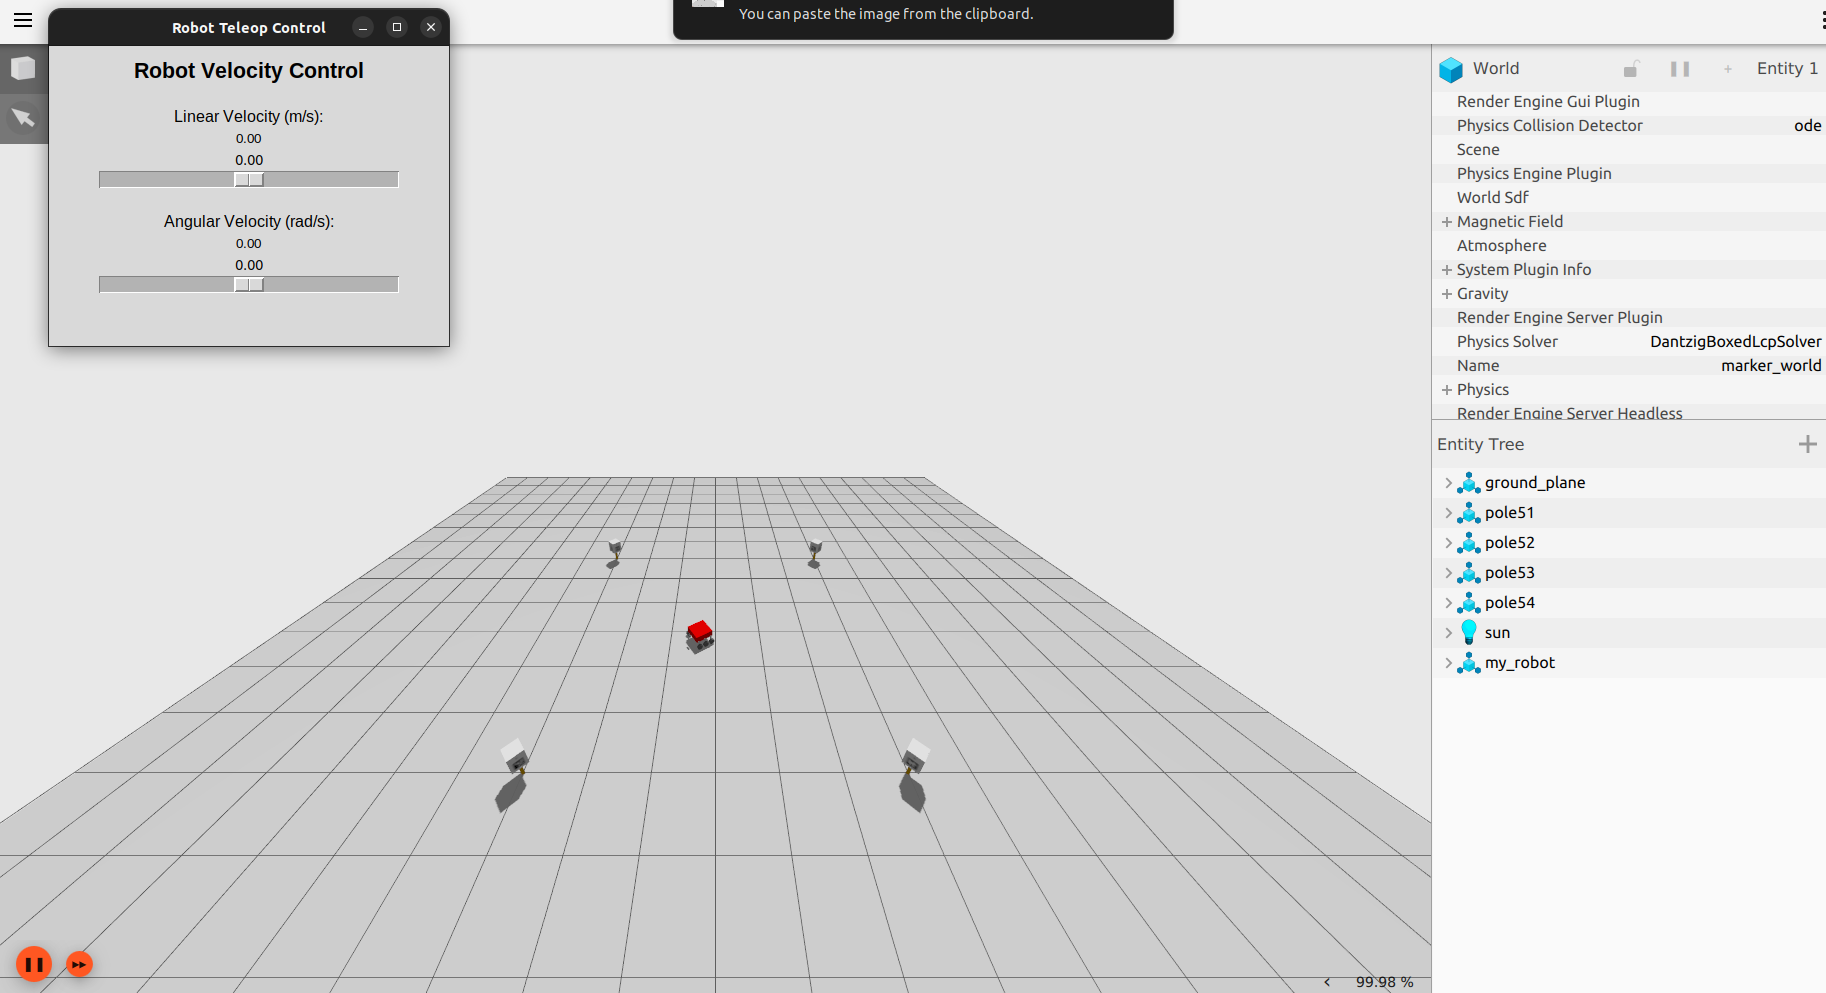
\includegraphics[width=0.98\textwidth]{gazebo.png}
    \caption{Gazebo simulation with the robot spawned in the marker world and the teleop GUI used during runtime testing.}
    \label{fig:gazebo_sim}
\end{figure}

\subsection{Runtime Verification and Topic Validation}

The terminal evidence is valuable because it confirms that the expected runtime graph came up cleanly: the robot state publisher, camera frame publisher, bridge nodes, RViz, and the ArUco detection node all launched together. The topic listing also shows that the perception pipeline is connected to the correct ROS names and that the detected marker data is flowing through the system.

\begin{figure}[h]
    \centering
    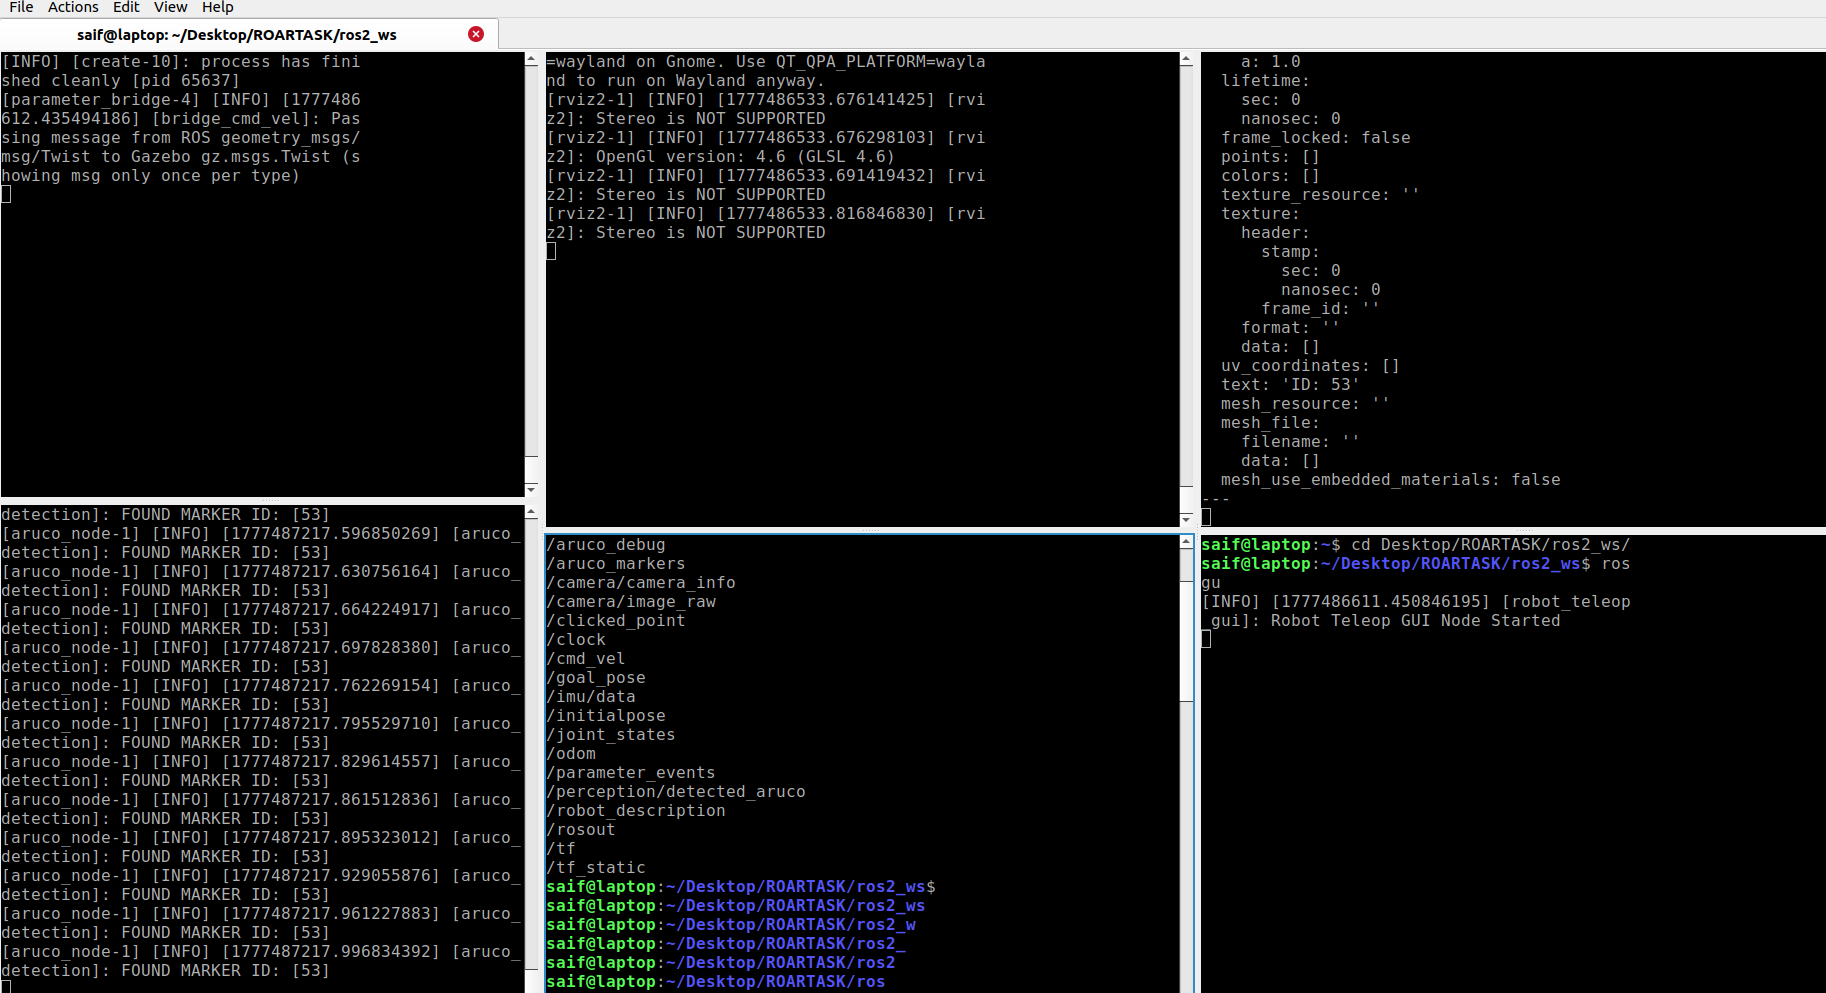
\includegraphics[width=0.98\textwidth]{terminal.png}
    \caption{Terminal verification showing active nodes, bridged topics, and ArUco marker detection output with ID 53.}
    \label{fig:terminal_validation}
\end{figure}

\subsection{TF Tree and RViz Debugging}

One of the more visible problems during validation was that the RViz model looked corrupted: the wheel links appeared stacked and RViz reported missing transforms for parts of the robot. The investigation showed that joint-state propagation was the weak point in the simulation pipeline, so the wheel and arm links were not being updated reliably. Once joint-state publication and the transform chain were restored, the model tree became complete and RViz could resolve the links correctly.

\begin{figure}[h]
    \centering
    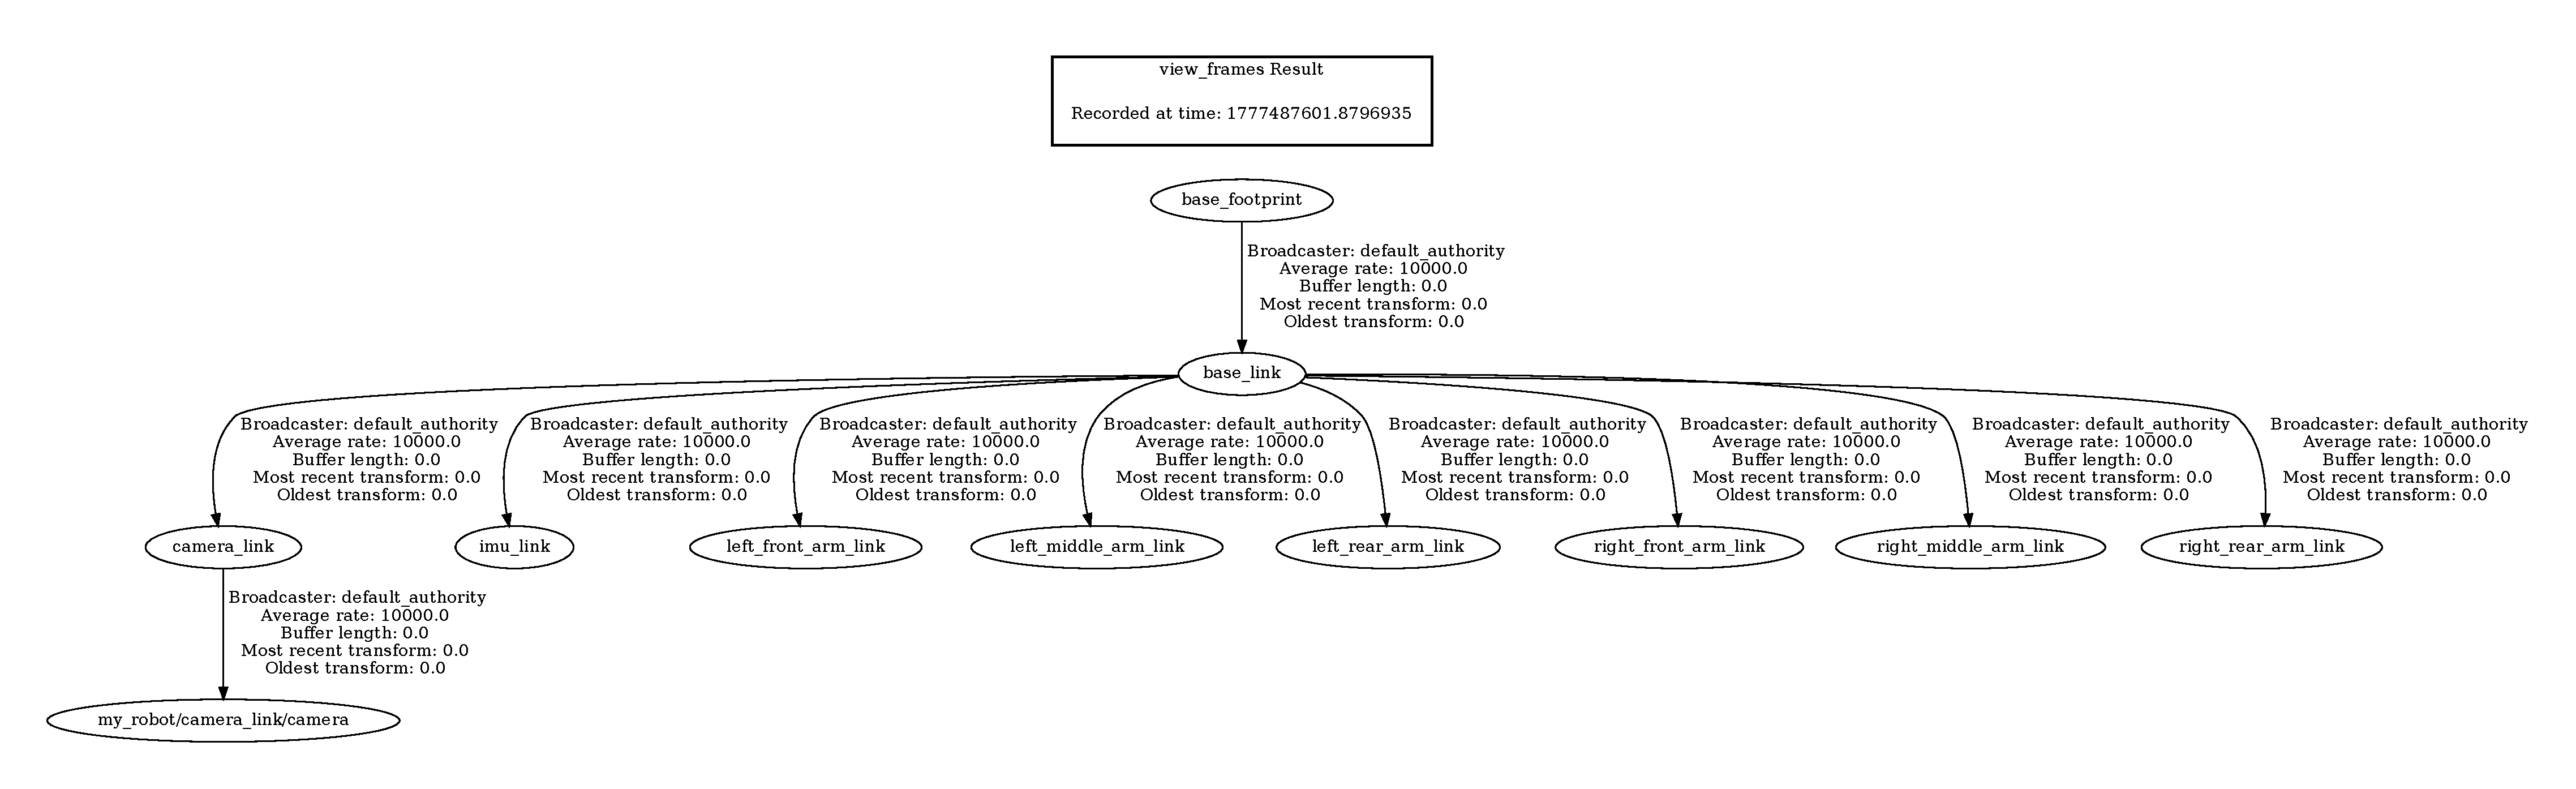
\includegraphics[width=0.98\textwidth]{frames_2026-04-29_21.33.21.pdf}
    \caption{TF tree exported from the running system after joint-state publication was restored.}
    \label{fig:tf_tree}
\end{figure}

\begin{figure}[h]
    \centering
    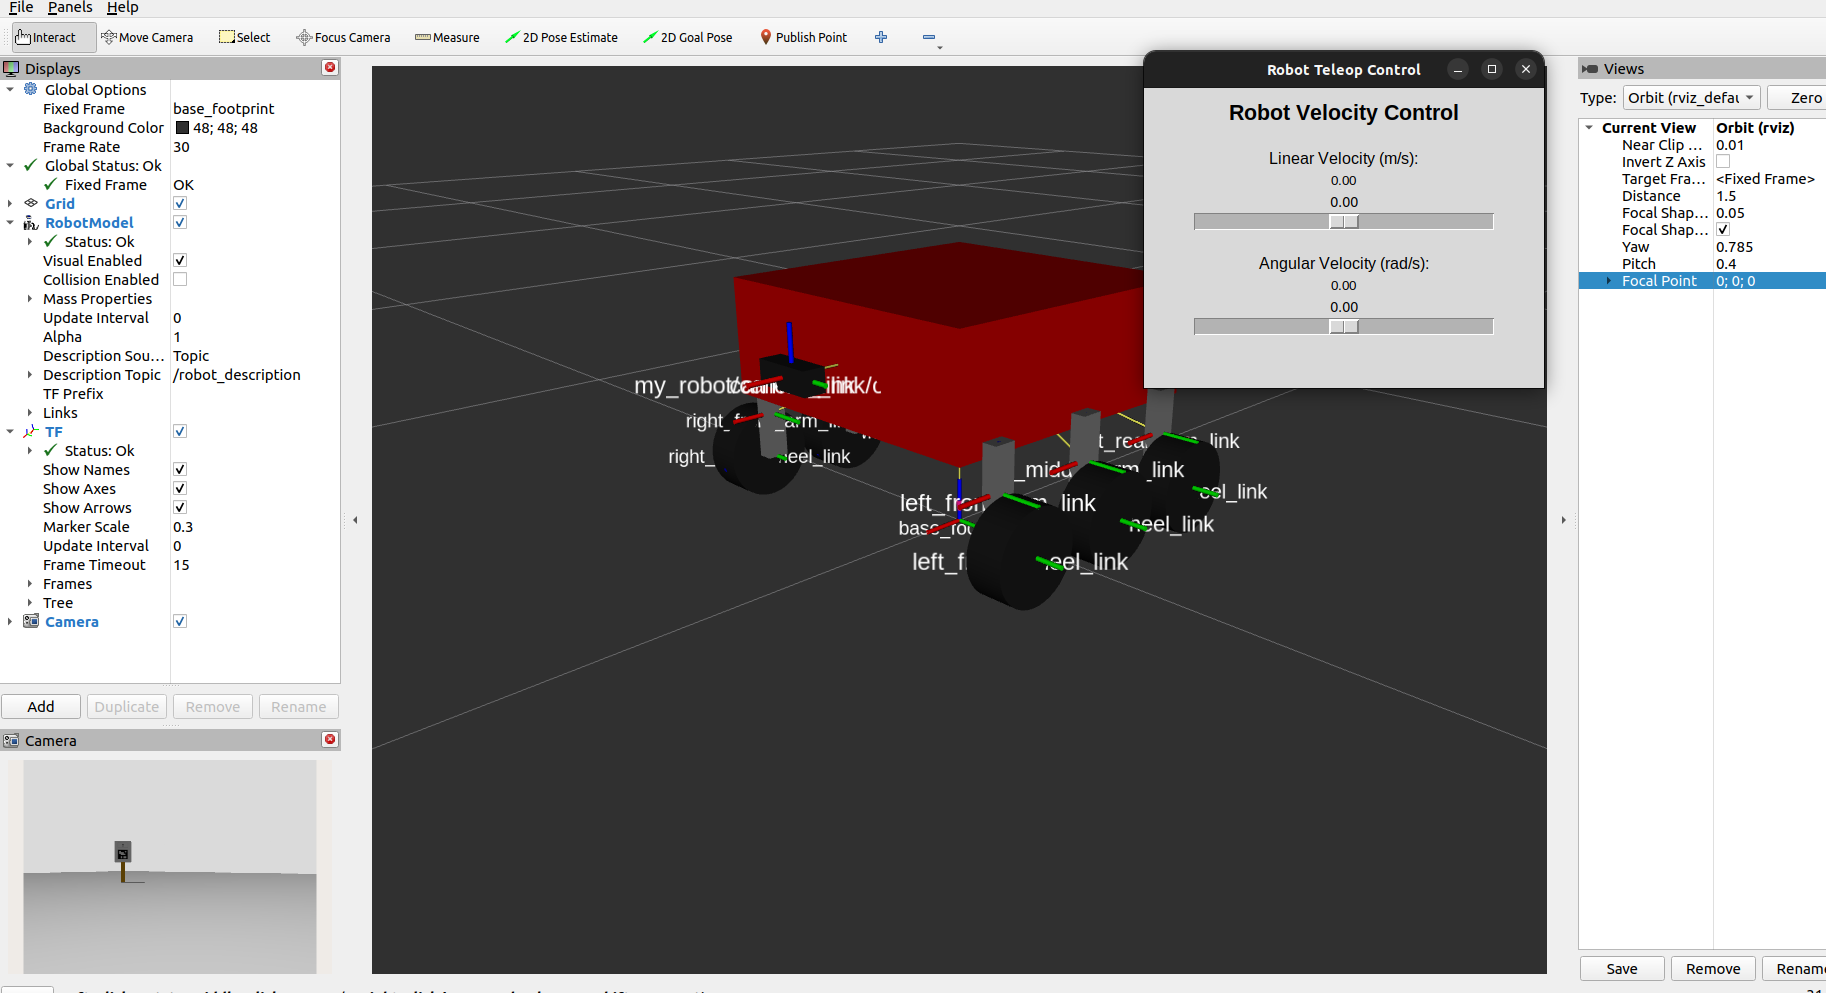
\includegraphics[width=0.98\textwidth]{Rviz.png}
    \caption{RViz model view after the transform issue was fixed and the wheel frames resolved correctly.}
    \label{fig:rviz_view}
\end{figure}

\subsection{ArUco Marker Detection and Tracking Node}

The core component of this task is the \texttt{aruco\_tracking} node, responsible for real-time identification of ArUco markers from the robot's camera feed.

\textbf{Methodology:}
I integrated the existing ArUco tracking stack with the robot camera feed through the launch and bridge configuration, so the marker results appear in the ROS tools without repeating the detector implementation itself in the report.

\textbf{Technical Highlights \& Code Strengths:}
\begin{itemize}[leftmargin=*]
    \item \textbf{Robust Message Conversion:} Seamless integration with \texttt{cv\_bridge} to confidently transfer data between ROS \texttt{Image} messages and image-processing data paths.
    \item \textbf{Dynamic Pose Estimation:} Accurate 3D pose estimation utilizing camera intrinsic matrices to provide continuous feedback of the markers' relative positions.
    \item \textbf{Clean System Architecture:} A highly modular Object-Oriented paradigm ensuring the node can be scaled and easily maintained.
\end{itemize}

Rather than repeating the detection algorithm itself, the report focuses on the implemented integration around it. The perception stack is launched by \texttt{aruco\_detection.launch.py}, which starts the existing \texttt{aruco\_tracking} node, sets \texttt{arucoDictType=7} and \texttt{markerSize=0.15}, and remaps the robot camera topics into the names the node expects. That makes the report reflect the actual engineering work in the workspace: wiring the detector into the simulation, not re-explaining the detection task that was already provided.

\subsection{Visualizing Output with GUI and RViz2}

To validate the node's performance, I implemented visualization techniques to display both the raw and annotated camera feeds, proving that the tracking system works successfully under simulated conditions. The validation flow followed the camera testing guide by checking \texttt{/camera/image\_raw}, \texttt{/camera/camera\_info}, RViz, \texttt{rqt\_image\_view}, and the camera verification script.

\begin{figure}[h]
    \centering
    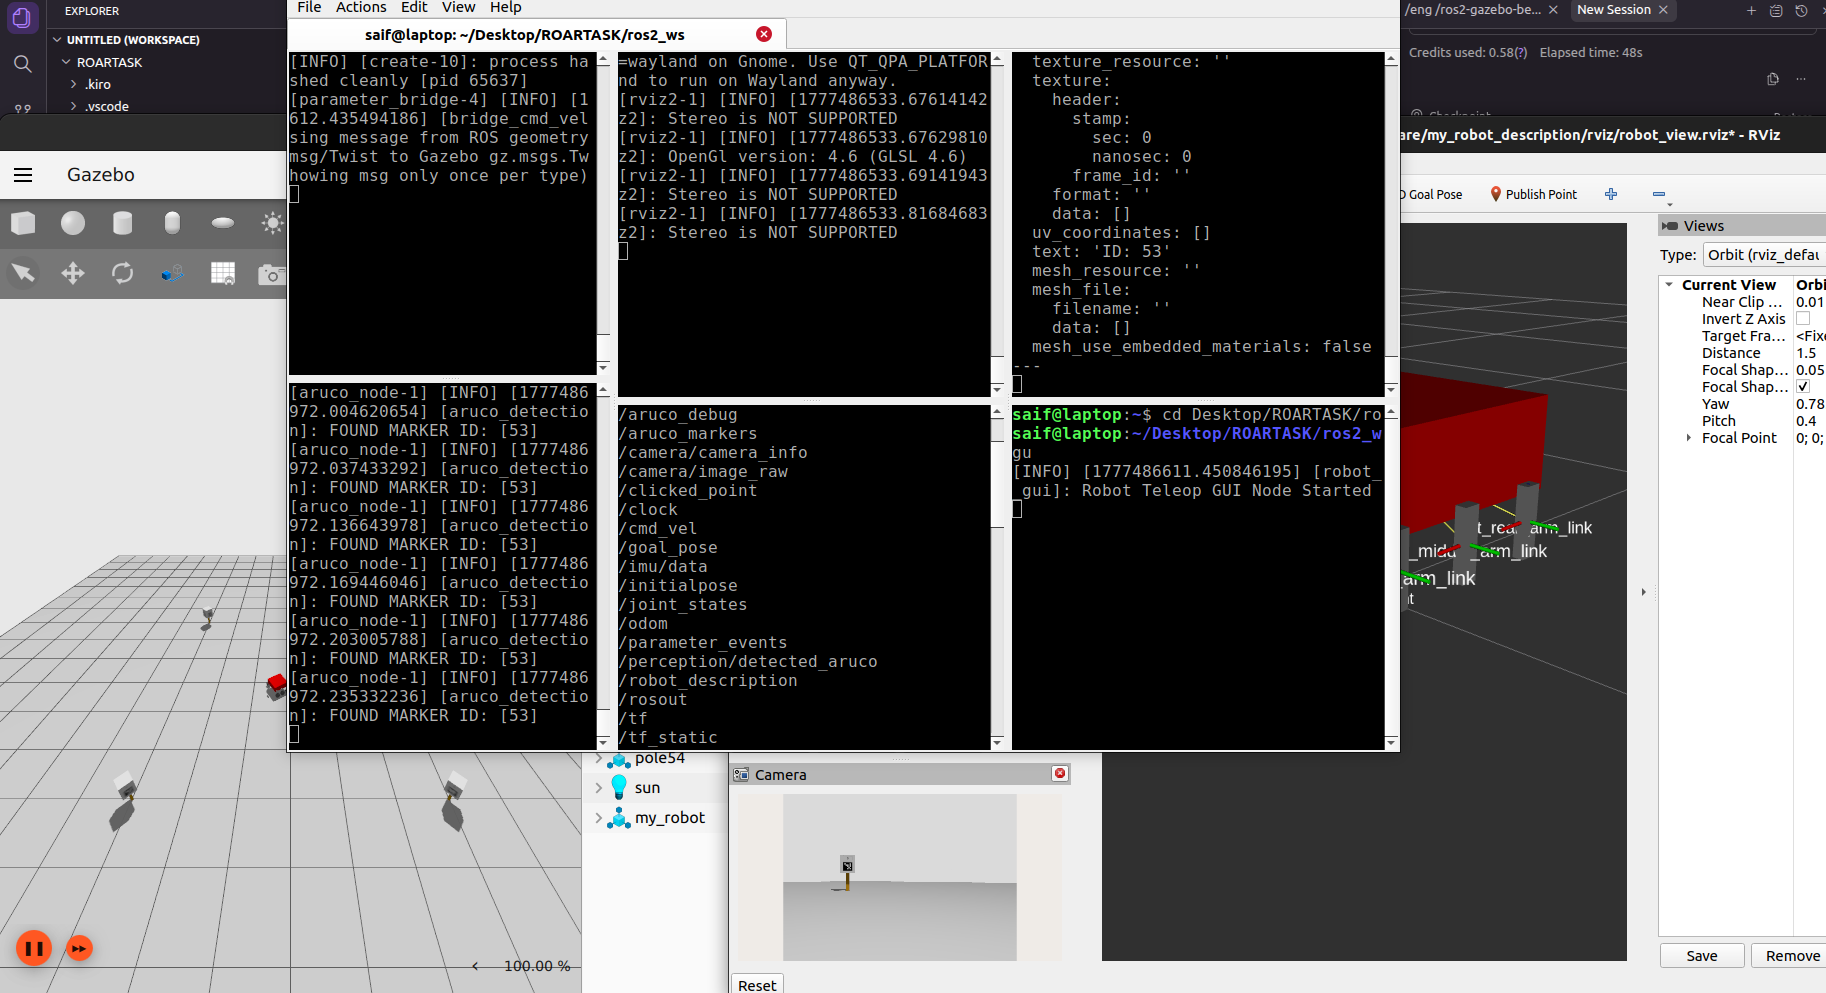
\includegraphics[width=0.98\textwidth]{1.png}
    \caption{Integrated system overview showing topic checks, node activity, ArUco detection output, RViz, Gazebo, and the map context in one capture.}
    \label{fig:aruco_detection}
\end{figure}

\textbf{Execution Details:} 
I utilized \texttt{rqt\_image\_view} and a custom \texttt{robot\_teleop\_gui.py} to ensure both manual control of the rover and real-time visualization of the tracking subsystem were successful. The implementation effectively handles varying lighting conditions and distances within the Gazebo engine.

\subsection{Additional Photos Showcasing the Working Project}

These extra captures provide additional evidence that the simulation, RViz, and perception pipeline were all operating together correctly.

\begin{figure}[h]
    \centering
    \begin{minipage}{0.48\textwidth}
        \includegraphics[width=\linewidth]{additional_photo_1.png}
    \end{minipage}
    \hfill
    \begin{minipage}{0.48\textwidth}
        \includegraphics[width=\linewidth]{additional_photo_2.png}
    \end{minipage}
    \caption{Additional photos showcasing the working project.}
\end{figure}

\begin{figure}[h]
    \centering
    \begin{minipage}{0.48\textwidth}
        \includegraphics[width=\linewidth]{additional_photo_3.png}
    \end{minipage}
    \hfill
    \begin{minipage}{0.48\textwidth}
        \includegraphics[width=\linewidth]{additional_photo_4.png}
    \end{minipage}
    \caption{Additional photos showcasing the working project.}
\end{figure}

\end{document}
